\documentclass[tikz]{standalone}
\usepackage{fontspec}
\renewcommand*{\familydefault}{\sfdefault}
\usepackage{standalone}
\usepackage{amssymb}
\usetikzlibrary{arrows.meta, decorations.pathreplacing, shapes.geometric}
%\usetikzlibrary{positioning,fit,shapes.geometric,fadings,bayesnet}

\begin{document}

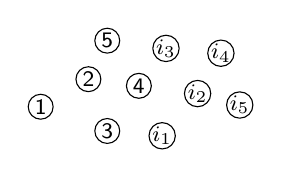
\begin{tikzpicture}
[font=\footnotesize, label distance=0 cm, inner sep=0.5 pt,
%every node/.style={anchor=center},
every node/.style={draw, inner sep=0 pt, minimum size=9 pt, circle, fill=none}
]

% position sites in schematic structure
%\draw[line width=4 pt, gray!30!white]
\path
(0,0) coordinate (a1)
-- ++(30:0.7) coordinate (a2)
-- ++(-70:0.7) coordinate (a3)
-- ++(55:0.7) coordinate (a4)
-- ++(125:0.7) coordinate (a5)
(a3) ++(-5:0.7) coordinate (a6)
-- ++(50:0.7) coordinate (a7)
-- ++(125:0.7) coordinate (a8)
-- ++(-05:0.7) coordinate (a9)
-- ++(-70:0.7) coordinate (a10)
;

% site labels
\path[draw] foreach \x in {1,...,5}
{(a\x) node (A\x) {\x}}
;
\path[draw] foreach \x/\y in {6/1,7/2,8/3,9/4,10/5}
{(a\x) node (A\x) {\(i_\y\)}}
;

\path
(A2) ++(110:0.3 cm) coordinate (B2a) ++(110:0.15 cm) coordinate (C2a)
(A2) ++(170:0.3 cm) coordinate (B2b) ++(170:0.15 cm) coordinate (C2b)
(A3) ++(220:0.3 cm) coordinate (B3a) ++(220:0.15 cm) coordinate (C3a)
(A3) ++(170:0.3 cm) coordinate (B3b) ++(170:0.15 cm) coordinate (C3b)
(A3) ++(-60:0.3 cm) coordinate (B3c) ++(-60:0.15 cm) coordinate (C3c)
%(A9) ++(220:0.3 cm) coordinate (B9a) ++(220:0.15 cm) coordinate (C9a)
(A10) ++(250:0.3 cm) coordinate (B10a) ++(250:0.15 cm) coordinate (C10a)
(A10) ++(200:0.3 cm) coordinate (B10b) ++(200:0.15 cm) coordinate (C10b)
;

\end{tikzpicture}

\end{document}
